\section{Sensorenhet}
Sensorenheten har i uppgift att läsa in sensordata och omvandla den till ett läsligt format. Se figur \ref{fig:unitSensor} för en övergripande systemskiss för sensorenheten.
\begin{figure}[h!]
    \makebox[\textwidth][c]{\includegraphics[width=0.6\textwidth]{sensorenhet.png}}
    \caption{Översikt över sensorenheten.}
    \label{fig:unitSensor}
\end{figure}

\noindent \begin{small}
    * Om I\textsuperscript{2}C används krävs även en logic level converter mellan 5V och 3V3 på dessa platser.\\
    ** 5V på Atmega-sidan, 3V3 krävs av sensorn.
\end{small}
\subsection{Hårdvara}

\subsubsection{Hårdvarolista}
Här listar vi upp all hårdvara som vi behöver för att sensorenheten ska fungera.
\begin{center}
	\begin{tabular}{|l|l|c|}
		\hline
		Komponent & Förklaring & Antal \\
		\hline\hline
		ATmega1284 & En mikroprocessor med 44 pinnar & 1 \\
		\hline
		SRF04 & Ultraljudssensor & 5 \\
		\hline
		LIDAR lite v2 & Lasersensor & 1 \\
		\hline
		MLX90609 & Gyro & 1 \\
		\hline
	\end{tabular}
\end{center}

\subsubsection{Processor}
ATmega1284 används som processormodell, då den är kraftfull utan att ta det till överdrift, men även har tillräckligt med avbrottsingångar för att kunna arbeta med LIDARn och samtliga ultraljudssensorer, se \ref{sssec:sonicsensors}.

\subsubsection{Ultraljudssensor} \label{sssec:sonicsensors}
\paragraph{Alternativ 1}
En ultraljudssensor, SRF04, placeras på var och en av robotens fyra sidor och används för navigering och positionsuppskattning. Dessa behöver en utgång och en interrupt-ingång var. Se \ref{ssec:sensorInterface}. Dessa kan användas var 65:e millisekund utan risk för störningar, vilket ger oss möjlighet att läsa av $\sim15$ sensorer per sekund. Troligtvis kan de även användas med mindre eller ingen marginal mellan avläsningarna, men det kräver testning för att avgöras. En annan nackdel är att de fungerar dåligt i vinkel mot en vägg, där de antingen inte ger något värde alls, eller ett ''studsat'' värde. %http://www.robot-electronics.co.uk/htm/sonar_faq.htm

\paragraph{Alternativ 2}
Som alternativ kan IR-sensorer användas. Nackdelen är störningar i den analoga utdatan, som dessutom är ickelinjär, och fungerar på ett kortare intervall än ultraljudssensorer. Fördelen är snabbare avläsningar som troligtvis inte stör varandra. Bredden på mätstrålen är också mindre än med ultraljud.


\subsubsection{LIDAR lite v2} \label{sssec:lidar}
LIDAR är en kraftfull lasersensor som i systemet som helhet används för mätningar som kräver noggranhet. Komponenten kan kommuniceras med via en trigger-pin och PWM-output, alternativt via en I\textsuperscript{2}C-buss. I första hand kommer PWM användas.

Sensorn monteras på toppen av roboten - ovanpå ett roterande servo, som specificeras i större detalj i avsnitt \ref{ssec:servomotor}. Detta för att effektivt kunna mäta avstånd i flera vinklar.

\subsubsection{IMU} \label{sssec:imu}

\paragraph{Alternativ 1}
En enklare modul - exempelvis MLX90609 - används, via en analog ingång. Detta ger oss då endast rotationen kring z-axeln, som kan användas för att beräkna robotens riktning i rummet.

\paragraph{Alternativ 2}
En mer avancerad modul, exempelvis MPU6050, används, via en I\textsuperscript{2}C-buss. Om LIDARn implementerats med I\textsuperscript{2}C delas bussen mellan dessa två. Det ger oss i så fall både riktning och acceleration, för att mer noggrannt kunna beräkna robotens placering.% TODO: MotionMagi, handledare

\subsection{Mjukvara}

Koden ska vara skriven i C, och ska följa standarden specificerad i bilaga \ref{sec:cstandard}.

Programmet ska omvandla sensordata till ett mer läsligt format, och ska kunna skicka det vidare (se \ref{ssec:sensorInterface}).

\subsection{Gränssnitt} \label{ssec:sensorInterface}
Sensorenheten kommer behöva kommunicera med de faktiska sensorerna, samt ha ett sätt att passera vidare utdata. Sensorenheten kan ta emot uppmaningar om att starta en avläsning via samma buss som används för att rapportera mätvärden vidare.

\subsubsection{LIDAR}
LIDAR kommer i första hand använda avläsningstriggers och PWM via en gemensam pin. PWM-signalen kopplas i så fall till ett avbrott för att mäta dess längd, som används för att beräkna avståndet. Som alternativ kan också I\textsuperscript{2}C användas.

\subsubsection{I2C-buss}
Den mer avancerade av IMUerna använder I\textsuperscript{2}C. Även LIDARn kan kommunicera via I\textsuperscript{2}C. Om behov uppstår implementerar vi en I\textsuperscript{2}C-buss. Vi stödjer i så fall inte flera masters, utan behandlar processorn som den enda, med LIDAR:n och gyron som slavar.

\subsubsection{Ultraljudssensorer}
Ultraljudssensorerna (\ref{sssec:sonicsensors}) använder ett liknande gränssnitt som LIDARn, med en trigger-pin och en echo-pin som utgång. Deras utvärde beror på längden av dess höga signal, så för att garantera att vi börjar mäta omedelbart på en hög flank så ska avbrott utnyttjas. Detta uppnås genom att helt enkelt koppla denna signal till en av avbrottsportarna på processorns, för var och en av sensorerna.

\subsubsection{Utvärden/Input}
Hur tas instruktioner emot, samt hur passeras processerade mätvärden vidare?

\paragraph{Alternativ 1}
Implementera en UART-buss som endast går mellan sensorenheten och kommunikationsenheten. Se \ref{ssec:brainInterface} för mer detaljer om för och nackdelar.

\paragraph{Alternativ 2}
I\textsuperscript{2}C-bussen som eventuellt används för att kommunicera med LIDAR:n och gyron kan utnyttjas, med även processorn som slav. Enheten som tar emot data från/skickar data till sensorenheten får istället ta över rollen som master. Se \ref{ssec:brainInterface} för mer detaljer om för och nackdelar.